\documentclass{beamer}
\usepackage[T1]{fontenc}
\usepackage[utf8]{inputenc}
\usepackage{ngerman}
\usepackage{amsmath,amsfonts,amssymb}
\usepackage{booktabs}
\usepackage{xcolor}
\usepackage{graphicx}
\usepackage[scaled=0.93]{helvet}
\usetheme{CambridgeUS}
\usecolortheme{beaver}
\setbeamercolor{itemize item}{fg=red}
\setbeamertemplate{itemize items}[square]
\setbeamertemplate{itemize item}[red]
\setbeamertemplate{blocks}[rounded][shadow=false]
\beamertemplatenavigationsymbolsempty

\newcommand{\ket}[1]{\left| #1 \right>} % for Dirac bras
\newcommand{\bra}[1]{\left< #1 \right|} % for Dirac kets
\newcommand{\braket}[2]{\left< #1 \vphantom{#2} \right|
\left. #2 \vphantom{#1} \right>} % for Dirac brackets
\newcommand{\vect}[1]{\boldsymbol{\mathbf{#1}}}


\title[Theory Group Seminar Talk]{\textbf{Diffusion Controlled Reaction Rates over Fluctuating Barriers}}
\author[J.Kolb]{Jakob J. Kolb}
\institute[HU-B: AG Soft Matter Theory]{Helmholtz-Zentrum Berlin\\Soft Matter Theory}
\date{24th January 2014}

\begin{document}


\frame[label=titlepage]{\titlepage}



\section{Introduction}

\frame{
    \begin{minipage}[t]{0.4 \textwidth}
        \begin{figure}[H]
            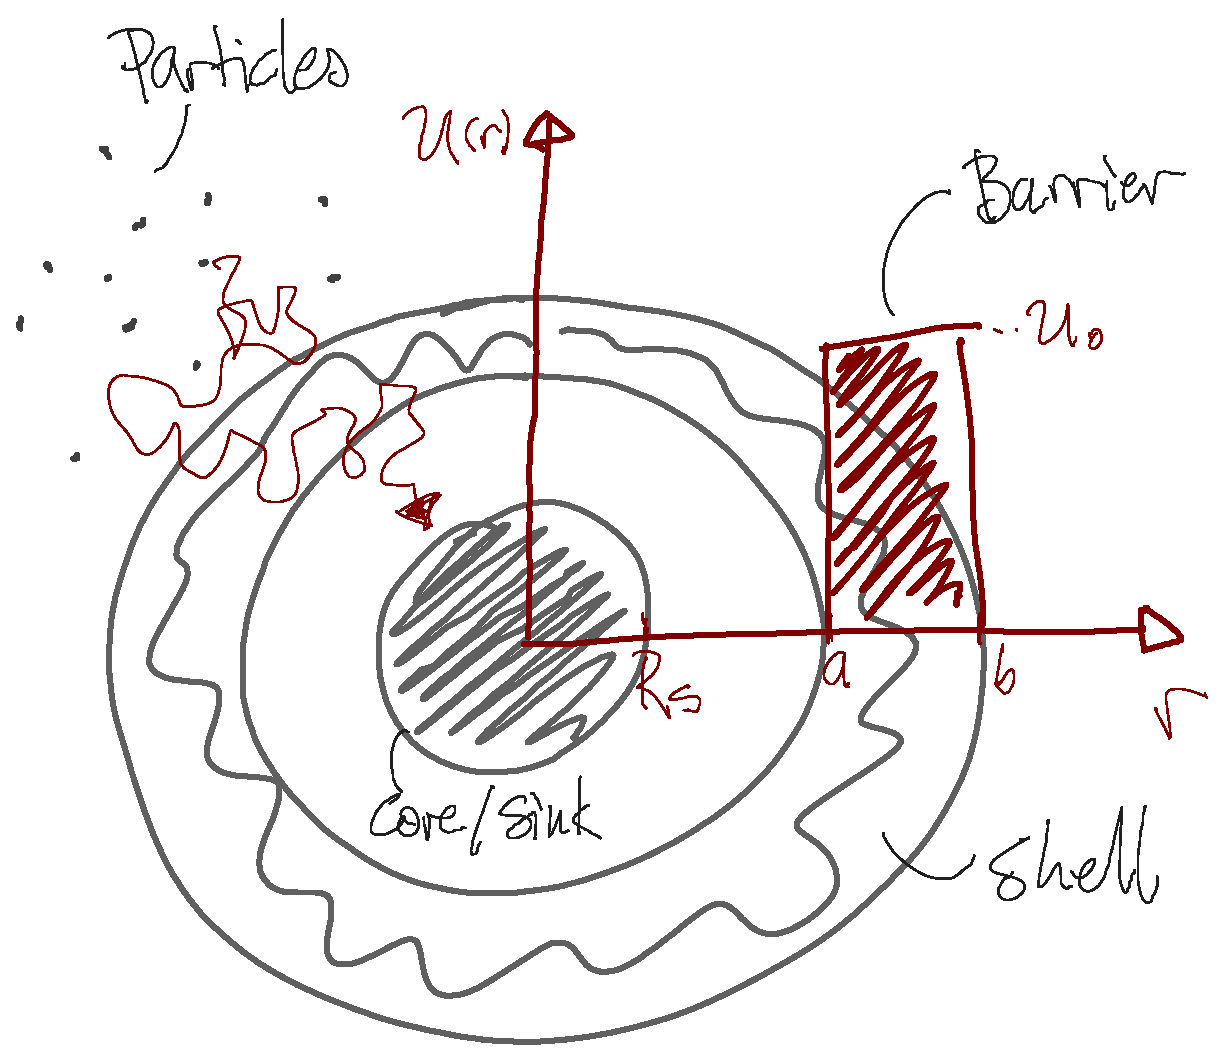
\includegraphics[width = 1 \textwidth]{skizze.eps}
        \end{figure}
    \end{minipage}\vspace{.05 \textwidth}\begin{minipage}[t]{0.55 \textwidth}
        \begin{align*}
            &\frac{d \vec{x}_i}{d t} = -\frac{1}{\gamma}\vec{\nabla}U_i(\vec{x}_i) + \sqrt{2D} \varepsilon(t)\\
            &U_i \in [U_0, \cdots, U_n] \\
            &\frac{d}{d t}\vect{P}_U = \hat{W}\vect{P}_U\\
        & Important \quad property \quad of \quad \hat{W}\\
            &\hat{W}\vect{\rho}^{(eq)} = 0, \quad W_{ij}\rho_{i}^{(eq)} = W_{ji}\rho_{j}^{(eq)}    
        \end{align*}
    \end{minipage}
    The resulting Fokker-Planck equation and boundary conditions are:
    \begin{align}
        &\frac{\partial \vect{\rho}}{\partial t} = \hat{\Gamma}_{FP}\vect{\rho} + \hat{W}\vect{\rho}  \\
        &\hat{\Gamma}_{FP} = {\rm diag}\left[ \vec{\nabla} U_{i}(\vec{r}) \vec{\nabla} + D \vec{\nabla}^{2} \right] \nonumber\\
        &\vect{\rho}(R_s) = 0, \quad \vect{\rho}(r \rightarrow \infty) = \vect{\rho}^{(eq)} \nonumber
        \label{FPE}
    \end{align}

}
\section{Solution}		
\frame{
    Fitting conditions at jump discontinuities of the potential in steady state
    \begin{align}
        &\int_{R_s}^{r}\hat{\Gamma}_{FP}\vect{\rho}(r'){\rm d} r' = - \hat{W} \int_{R_s}^{r} \vect{\rho}(r') {\rm d} r' \nonumber \\
        &\frac{1}{\gamma}\rho_i(r) \vec{\nabla} U_i(r) + D \vec{\nabla} \rho_i(r) = J_i(R_s) - \left\{ \hat{W} \int_{R_s}^{r} \vect{\rho}(r') {\rm d} r' \right\}_{i} \nonumber \\
        &\int_{a-\varepsilon}^{a + \varepsilon} \frac{U_i}{\gamma D}\delta(a-r) + \int_{a-\varepsilon}^{a + \varepsilon} \frac{1}{\rho_i(r)}\nabla \rho_i(r) = \underbrace{\int_{a - \varepsilon}^{a + \varepsilon}\frac{J_i(r)}{\rho_i(r) D} - \int_{a - \varepsilon} ^{a+ \varepsilon} \left\{ \hat{W} \vect{n}(r)\right\}_{i}}_\text{$O(\varepsilon)$} \nonumber 
    \end{align}
    So in the limit of $\varepsilon \rightarrow 0$ we have:
    \begin{equation}
        \vect{\rho}^{I} =  {\rm diag}\left[\exp\left\{\frac{U_i}{K_B T} \right\}\right] \vect{\rho}^{II}
    \end{equation}
    }

\section{Modell}

\frame{
\frametitle{\textbf{Modell}}
	
}




\subsection{Lösungsweg}

\section{Ergebnisse}

\frame{
\frametitle{\textbf{Lösungsmethoden}}
\begin{itemize}
	\item gekoppeltes Differentialgleichungssystem $\rightarrow$ Dipol-Dipol-Korrelationsfunktion
	\item Fouriertransformation $\rightarrow$ Absorption
	\item analytische Lösung
		\begin{itemize}
			\item Greensche Funktionen
			\item Exzitonenzustände müssen bekannt sein
		\end{itemize}
	\item numerische Lösungsweg
		\begin{itemize}
			\item Integration (z.B. Runge-Kutta)
			\item Fast Fourier Transform
		\end{itemize}
\end{itemize}
}
\subsection{Parameter}
\frame{
\frametitle{\textbf{Parameter}}
\begin{tabular}{l c c}
\toprule
Anzahl d. Moleküle pro Kette & $N$ & 10 \\
Übergangsdipolmoment d. Moleküle & $d_m$ & 8 D\\
Intermolekularer Abstand & $\Delta x_{mol}$ & 1.2 nm\\
Energie d. ersten angeregten Zustands & $E_m$ & variiert um $E_N$\\
Radius d. MNP & $a$ & 10 nm\\
Übergangsdipolmoment des MNP & $d_N$ & 2925 D\\
Plasmonenergie & $E_N$ & 2.6 eV\\
\bottomrule
\end{tabular}
}










\subsection{Ausblick}


\subsection{Zusammenfassung}
\frame{
\frametitle{\textbf{Zusammenfassung}}
\begin{itemize}
	\item 
	\item 
	\item 
		\begin{itemize}
			\item 
		\end{itemize}
	\item 
\end{itemize}
}






\end{document}


